%%%%%%%%%%%%%%%%%%%%%%%%%%%%%%%%%%%%%%%%%%%%%%%%%%%%%%%%%%%%%%%%
\begin{comment}

* Maintain 80 characters / line.
 
* too much ``''s make the sentence look scattered and visually less recognizable. ``e.g.'' also.

* \em, \bf, \it are all obsolete \TeX primitives, and it does not take effect properly --- for example, {\bf {\it aaa}} shows ``aaa'' in italic but NOT IN BOLD. Use \emph{}, \textit{}, \textbf{} and so on.

* always use \ff, \fd, \cea, \pr, \mv , and do not use it directly, e.g. FF, FD/LAMA2011, etc. 

* use of footnotes should be minimized.

* IPC2011 should always be \ipc . The definition can later be modified in abbrev.sty .

* prefer separated words over hyphened words. domain
  independent>domain-independent, planner independent >
  planner-independent.

* Table, Figure, Fig., should not be used directly. Always use \refig and \reftbl. When the development flag is enabled, direct use of \ref signals an error.

* Caption ends with a period.
\end{comment}

%%%%%%%%%%%%%%%%%%%%%%%%%%%%%%%%%%%%%%%%%%%%%%%%%%%%%%%%%%%%%%%%

\begin{abstract}
% % intentionally made different from the 1st-order symbol paper, writing style is also different
% While domain-independent classical planning is an active area of research,
% its applicability to the real-world tasks are limited to those precisely modeled by human.
% Recently, \latentplanner \cite{Asai2018} combined classical planning with deep-learning
% to obtain the symbolic description of the image based domain.
% In this paper, we address a problem in their preliminary implementation of \latentplanner,
% specifically the uninformative / random propositions in the latent / symbolic encoding,
% and provides a remedy for it.
% %
% Those uninformative propositions become true or false depending on the coin flip,
% which means that
% % some of the propositiosn in the latent layer may not carry significant meaning / affect the output.
% % While this is not problematic for encoding/decoding, from search/planning perspective this is a major problem,
% % because this means that 
%  a single state can have multiple propositional representations and no longer the
% unique representation amenable for search algorithms.
% % 
% One effective way to suppress this behavior is to have an additional regularization
% for the latent propositions which guides the training so that 
% % toward sparser, disentangled propositional representation,
% unused propositions tends to be 0.
%  % 
% We empirically show that this ``Zero-Suppressed SAE''
% has lower variance encoding (more stable propositions) for each single state
% and improves the success rate of \latentplanner.
% % XXX TODO: unknown if it is possible
% [TODO]
% Furthermore, we show that this Zero-Suppressed SAE can act like a declarative knowledge base
% where you incrementally assign new knowledge to unused propositions.
% We show this by retraining an existing network
% with a mixture of the existing and new dataset, and demonstrating that
% it can encode both environments.
While Classical Planning is an active branch of AI,
its applicability is limited to the tasks precisely modeled by humans.
Fully automated high-level agents should be instead able to find a symbolic representation
of an unknown environment without supervision,
% i.e., no help from
% manually-assigned labels nor predefined reinforcement signals,
otherwise it exhibits knowledge acquisition bottleneck.
% 
Meanwhile, \latentplanner \cite{Asai2018} uses a Neural Network (NN)
called State AutoEncoder (SAE) to obtain the propositional
representation of the image based puzzle domains with unsupervised learning,
then generates a propositional state space and performs Classical Planning,
partly resolving this bottleneck.
% 
In this paper,
we identify the problematic behavior of SAE-produced propositions 
as a new sub-problem of symbol grounding problem called the symbol \emph{stability} problem (SSP).
Informally, symbols are
\emph{stable} when their referents do not change against small perturbation in the environment,
and unstable symbols are harmful for symbolic reasoning.
We analyze the SSP in SAE
and propose ``Zero-Suppressed SAE'' (ZSAE), an enhancement of SAE that uses the idea of closed-world
assumption as a prior for NN optimization and improves the stability of the propositional variables.
% 
We empirically show that it finds more stable propositions as well as more compact representations
against various hyperparameters and improves the success rate of \latentplanner.
\end{abstract}


\section{Introduction}

% [This second version of introduction is too long]

Symbol grounding problem \cite{harnad1990symbol,Steels2008} is one of the key milestones in AI research
which seeks to achieve high-level intelligence.
% In Physical Symbol Systems Hypothesis \cite{newell1976computer}, it is believed that
% an agent with high-level intelligence performs tasks by efficiently manipulating a compact set of abstract symbols.
% 
% Symbolic manipulation
%  % consists of mechanical applications of composable rules which 
% allows for
% development of highly optimized and generalized, domain-independent heuristics (e.g. FF \cite{Hoffmann01} or LMcut \cite{Helmert2009})
% that can be easily applied to multiple tasks with few or no data,
% while the current learning-based approaches struggle to improve its multi-task performance and data efficiency.
% For example, training AlphaGo \cite{alphago} takes days on a huge cluster of custom-made Tensor Processing Units.
% % 
% To enable such a fully automated high-level symbolic computation in a real-world environment,
% agents should be able to find the symbolic representation of the environment by itself, i.e. solving the symbol grounding problem.
% 
Recently, Latplan system \cite[\refig{fig:overview}]{Asai2018} successfully
connected a subsymbolic neural network system and a symbolic Classical Planning system
to solve various visually presented puzzle domains.
% In contrast to the work by Konidaris et. al. (\citeyear{KonidarisKL14}),
% Latplan is a straightforward NN built upon a \lsota framework.
The State AutoEncoder (SAE) neural network in \latentplanner
generates a set of propositional symbols from the training images with no additional information,
and provides a bidirectional mapping between images and propositional states.
% 
The system then solves the propositional planning problem using a classical planner Fast Downward \cite{Helmert04}
and returns an image sequence that solves the puzzle
by decoding the intermediate propositional states of the plan.
It also discovers a set of action symbols that distinguish the modes of
state transitions through AMA$_2$ unsupervised learning process.
Therefore, the system grounds two kinds of symbols:
Propositional symbols and action symbols.
% 
The system opens a promising direction for applying a variety of symbolic methods to the real world.
The search space generated by \latentplanner was shown to be compatible
to an existing Goal Recognition system \cite{amado2018goal}.
Another approach replacing SAE/AMA$_2$ with InfoGAN was also proposed recently \cite{kurutach2018learning}.
% although it lacks the ability to find a finite set of action labels and resort to sample the successor states
% without guaranteeing to enumerate the successors.

Despite its success,
the propositional representations learned by SAE have a problematic behavior
because NNs in general do not have strong guarantees on the learned results.
They are not always ``stable'', i.e.,
some propositions may flip the value (true/false) randomly
given the identical or nearly identical image input.
% only slightly perturbed image input.
% 
% Prevent reviewers from reaching the early conclusion that this is about robustness.
% 
Curiously, instability does not affect the output accuracy of SAE.
This indicates that \emph{unstable} propositions are also ``unused'' and ``uninformative'',
just as the boy who cried wolf was ignored by the villagers.
 % in the Aesop's Fables.

Unstable symbols are harmful for symbolic reasoning because
they break the identity assumption built into the reasoning algorithms.
For instance, in \latentplanner, 
a single image may map to multiple propositional states due to stochasticity,
therefore the duplication detection in search algorithms such as \astar \cite{hart1968formal}
fails to realize that a single real-world state is visited multiple times through
different symbolic state representations.

\begin{figure}[tb]
 % It is better to have this figure in the first page --- whatever figure it is, it hooks
 % reader's interest
 \centering
 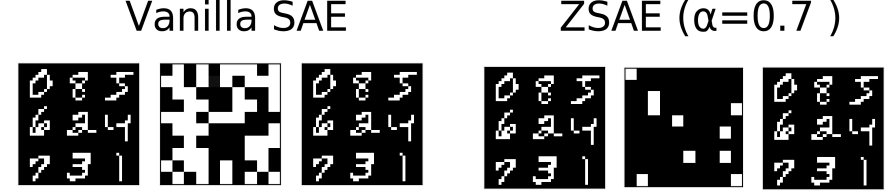
\includegraphics{img/zsae-overview.pdf}
 \caption{
Autoencoding results of an MNIST 8-puzzle state
using a vanilla State AutoEncoder (SAE) \cite{Asai2018} and a Zero-Suppressed SAE (ZSAE) with 100 propositions.
ZSAE obtains a compact representation that has fewer true bits.}
 \label{zsae-overview}
\end{figure}

% This problem arises for any grounding processes applied to the real world.
The first contribution of this paper is the identification of a sub-problem of symbol grounding
called ``symbol \emph{stability} problem'' (SSP), which seeks to find a set of symbols
whose values/referents are stable.
Stability is orthogonal to the \emph{performance/accuracy} of NNs:
NNs are known to robustly predict the correct output, but they do not guarantee
the quality of the internal representation.

The second and more concrete contribution of this paper is
the proposal of Zero-Suppressed State AutoEncoder (ZSAE, \refig{zsae-overview}).
ZSAE obtains a more ``stable'' propositions
by an additional penalty function which
guides the network optimization so that unused propositions tend to 
take the value of zero (false) instead of random values.
% 
The stable representation results in a higher success rate of classical planning.
Also, the network is less sensitive to the network size (hyperparameters)
as it automatically reduces the number of bits being used.
Moreover, we show that we can reduce the memory usage of the network
by pruning some unused neurons
that now have a constant activation of zero instead of random values.

% The rest of the paper is organized as follows.
% In \refsec{background}, we introduce Latplan \cite{Asai2018} and its SAE.
% Next, we describe a problematic behavior of this vanilla SAE and
% a broader problem of \emph{Symbol Stability Problem} (\refsec{issues}).
% We next analyze the vanilla SAE to understand the source of this behavior (\refsec{analysis}).
% Next, we introduce Zero-Suppressed SAE (ZSAE), the main contribution of this paper that addresses this problem (\refsec{zsae}).
% We empirically evaluate the stability of the propositions generated by the vanilla SAE and the ZSAE,
% as well as various other advantages of ZSAE (\refsec{evaluation}).
% We finally conclude the paper with related work and future remark (\refsec{conclusion}).


\section{Preliminaries}
\label{background}

\textbf{Symbol grounding} is an unsupervised process of establishing a mapping
from huge, noisy, continuous, unstructured inputs
to a set of compact, % clean
discrete, identifiable (structured) entities, i.e., symbols \cite{Asai2018}.
For example, PDDL has six kinds of symbols: Objects, predicates, propositions, actions, problems and domains.
Each type of symbol requires its own mechanism for grounding.
For example, the large body of work in the image processing community on recognizing 
objects (e.g. faces) and their attributes (male, female) in images, or scenes in videos (e.g. cooking)
can be viewed as corresponding to grounding the object, predicate and action symbols, respectively.
In this paper, we focus on the grounding process for propositional symbols.

\textbf{\latentplanner} \cite{Asai2018} is a framework for
\emph{domain-independent image-based classical planning}.
\latentplanner addresses two of the 6 types of symbols, % listed in \reftbl{tab:type-of-symbols},
namely propositional and action symbols.

Classical planners such as FF \cite{Hoffmann01} or
FastDownward \cite{Helmert04} takes a PDDL model as an input, which
specifies the state representation, the initial state, the goal
condition and the transition rules in the form of first order logic
formula.  In contrast, \latentplanner learns the state representation as well as the transition rules
entirely from the image-based observation of the environment with deep NNs.
% , and also claims to extend its capability on text/audio-based dialog data in the future.
The system was shown to solve various puzzle domains, such as 8-puzzles or Tower of Hanoi,
which are presented in a form of noisy, continuous visual depiction of the environment.

\begin{figure}[tb]
 \centering
 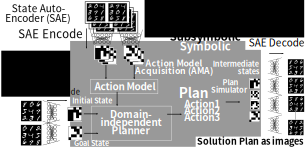
\includegraphics[width=\linewidth]{img/planning.pdf}
 \caption{Classical planning in latent space:
It uses the learned State AutoEncoder (\refig{sae}) to convert pairs of images $(\before,\after)$ to symbolic transitions,
 from which the Action Model Acquisition (AMA) component generates an action model.
A classical planner finds the symbolic solution plan for symbolic initial/goal states encoded from images.
Finally, intermediate states in the plan are decoded back to a human-comprehensible image sequence.}
\label{fig:overview}
\end{figure}

\latentplanner (\refig{fig:overview}) takes two inputs.
The first input is the \emph{transition input} $Tr$, a set of pairs of raw data.
Each pair $tr_i=(\before_i, \after_i) \in Tr$ represents a transition of the environment before and after some action is executed.
The second input is the \emph{planning input} $(i, g)$, a pair of raw data, which corresponds to the initial and the goal state of the environment.
The output of \latentplanner is a data sequence representing the plan execution that reaches $g$ from $i$.
While the original paper uses an image-based implementation (``data'' = raw images),
the type of data is arbitrary as long as it is compatible to NNs.

% Emphasize the type of symbol, as readers are not familier with or haven't deeply thought about symbols
% \subsection{SAE for Propositional Symbol Grounding}

\latentplanner works in 3 phases.
In Phase 1, a \emph{State AutoEncoder} (SAE) (\refig{sae}) learns a bidirectional mapping between raw data (subsymbolic representation e.g., images)
 and propositional states (symbolic representation) from a set of unlabeled, random snapshots of the environment.
% The $Encode$ function maps images to propositional states, and $Decode$ function maps the propositional states back to images:
The trained SAE provides two functions:
\begin{itemize} %this is crucial to understanding the rest of the paper, so making an itemize to highlight it
\setlength{\itemsep}{-0.3em}
\item $b=Encode(r)$ maps an image  $r$ to a boolean vector $b$.
\item $\tilde{r}=Decode(b)$ maps a boolean vector $b$ to an image $\tilde{r}$.
\end{itemize}
After training the SAE from $\braces{\before_i, \after_i\ldots}$,
it applies $Encode$ to each $tr_i \in Tr$ and obtain $(Encode(\before_i),$ $Encode(\after_i))=$ $(s_i,t_i)=$ $\overline{tr}_i\in \overline{Tr}$,
the symbolic representations (latent space vectors) of the transitions.

In Phase 2, an Action Model Acquisition (AMA) method learns an action model (e.g. PDDL, successor function) from $\overline{Tr}$ in an unsupervised manner.
The original paper proposed two approaches: AMA$_1$ is an oracle which directly generates a PDDL without learning,
by allowing it to use the whole set of valid transitions as an oracle.
In contrast, AMA$_2$ approximates AMA$_1$ by an unsupervised learning from examples.

In Phase 3, a planning problem instance is generated from the planning input $(i,g)$.
These are converted to symbolic states by the SAE, and the symbolic planner solves the problem.
For example, an 8-puzzle problem instance consists of an image of the start (scrambled) configuration of the puzzle ($i$), and an image of the solved state ($g$).

Since the intermediate states comprising the plan are SAE-generated latent bit vectors, the ``meaning'' of each state (and thus the plan) is not clear to a human observer.
However, in the final step, \latentplanner obtain a step-by-step visualization of the plan execution
by $Decode$'ing the latent bit vectors for each intermediate state.
This necessitates the bidirectionality of the mapping between the input and the propositional states.

\begin{figure}[tb]
 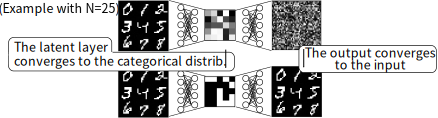
\includegraphics[width=\linewidth]{img/train-state-ae.pdf}
 \caption{Step 1:
Train the State AutoEncoder by
 minimizing the sum of the reconstruction loss and the variational loss of Gumbel-Softmax.
As the training continues, the output of the network converges to the input images.
Also, as the Gumbel-Softmax temperature $\tau$ decreases during training,
the latent values approach either 0 or 1.}
 % \caption{State AutoEncoder, a
 % Variational AutoEncoder \cite{kingma2014semi} using Gumbel-Softmax \cite{jang2016categorical} reparametrization in its
 % latent layer.}
 \label{sae}
\end{figure}

\subsection{SAE as a Variational AutoEncoder using Gumbel-Softmax}

The key concept of the SAE in \latentplanner is the use of Gumbel-Softmax \cite{jang2016categorical}
reparameterization trick in the latent activation of variational autoencoder~(VAE).
This allows SAE to obtain the
discretized binary representation, and \latentplanner uses this
discrete vector as the state representation for classical planning.
Below, we briefly review the literature.

An autoencoder~(AE)~\cite{hinton2006reducing} is a feed-forward NN that consists a pair of encoder and decoder networks, both of which are modeled by continuous functions.
AEs are trained so that the encoder maps a data point~(e.g., an image) into the low-dimensional latent space, and the decoder pulls the latent representation of the input back to the original data point.
Technically, they are trained by backpropagation so as to minimize the reconstruction loss, the distance between the input and the output measured by Euclidean distance or binary cross entropy (BCE).
Since the encoder is modeled by a continuous function, its latent representation is also continous, which makes it difficult to integrate AEs with propositional reasoners.
\if0
Since it is trained solely by the raw input data, it is a unsupervised learning method that do not require the human-assigned labels.
Its intermediate layer (typically smaller than the input) has a compressed, \emph{latent representation} of the input.
% AEs are commonly used for pretraining a NN.
NNs, including AEs, typically have continuous activations and integrating them with propositional reasoners is not straightforward.
\fi

A variational autoencoder~(VAE)~\cite{kingma2013auto} is a probabilistic vairant of AEs, where both encoder and decoders are modeled by probabilistic distributions.
By modeling the encoder by a Gumbel-Softmax distribution~\cite{jang2016categorical}, which approximates a discrete distribution, we are able to obtain a discrete latent representation of data.
VAEs are trained by backpropagation with the help of the reparameterization trick, which allows us to differentiate random variables.

% that forces the \emph{latent layer} (the most compressed layer in the AE) to follow a certain distribution (e.g., Gaussian).
% While initially proposed for enforcing Gaussian distributions, VAEs have been used to enforce arbitrary types of distribution (notably by Generative Adversarial Network \cite{goodfellow2014generative,makhzani2015adversarial}). 

In vanilla SAEs \cite{Asai2018}, the output layer of the encoder consists of $N$ units of Gumbel-Softmax
that approximates the Bernoulli distribution, %, resulting in a $N\times 2$ matrix,
and therefore, the latent representation can be regarded as $N$ binary propositional variables.


\if0
\subsection{Regularization in Neural Networks}

\emph{Regularization} is an important and broad concept in machine learning
that limits the representation capacity of a machine learning model by adding a constraint
so that the model better adapt to the underlying characteristics of the dataset.
% Regularization trades the training performance with generalization capability (testing performance, robustness to
% unseen data points) in order to suppress overfitting.
Regularization could be implemented in various ways.

One way is to designing the network topology for a particular data,
such as Convolutional Networks for images
or Recurrent Networks for sequential data, or
Dropout \cite{srivastava2014dropout}, that randomly drops some neurons so
that each pattern is more strongly associated with a fewer set of nodes.

Another way is to add a penalty term to the optimization metric of the
NNs that is minimized by the optimization algorithms such as Stochastic Gradient Descent.
Common regularization techniques in this category include
$l_1$ (LASSO) or $l_2$ (ridge) regularization that respectively penalizes the absolute / square sum of the
activations or weights.
\fi
% It is necessary for the mapping to be bidirectional, because the
% propositional variables are machine-generated symbols, and also the
% resulting plan (returned as a sequence of propositional states) should
% be decoded back to real-world images which are interpretable for humans.

% \latentplanner also learns the action model using a neural action model acquisition method AMA$_2$,
% but we omit the details due to space limitation.

\section{Symbol Stability Problem}
% \section{Issues in the State Representation\\ in the vanilla SAE}
\label{issues}

SAE in \latentplanner can map a visual observation of the environment to/from a set of propositional values.
An issue in vanilla SAEs is that the class probability $\pi$ that is used inside its Gumbel-Softmax could be
neutral for the class ``true'' and the class ``false'' at some neuron,
causing the value of the neuron to change frequently (\refig{unstable}).
The source of stochasticity is twofold.
Firstly, the encoder is a probabilistic distribution, rather than a deterministic function.
%which includes a uniform random distribution.
This causes the propositions to change values even for the exact same inputs.
Secondly, the input image may be corrupted by a noise (stochastic observations)
while humans regard them as the ``same'' image.
When the class probabilities are neutral,
such a tiny variation in the input image may cause the activation to go across the decision boundary for each neuron,
causing the bit flips.

\begin{figure}[tb]
 \centering
 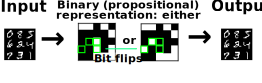
\includegraphics{img/unstable.pdf}
 \caption{Propositions found by SAEs may contain uninformative bits
 that flip randomly and do not affect the output.}
 \label{unstable}
\end{figure}

This stochastic behavior of the propositional representation
causes several serious problems from the classical planning point of view.
% 
Firstly, search algorithms that run on the state space generated based on these propositional vectors
are confused by many variations of the essentially identical real world states.
It could visit the same real world state several times because
the state may be encoded into different propositional vectors
and the duplicate detection in the search algorithm (e.g. \astar) falsely believes that they are separate.
% since it completely relies on the atomiticy and deteminisim of the proposition.
This slows down the search by increasing the number of nodes that are reachable from the initial state.

\begin{figure}[tb]
 \centering
 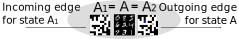
\includegraphics{img/disconnected.pdf}
 \caption{Random variations of propositional encoding for a single real-world state could disconnect the search space.}
 \label{disconnected}
\end{figure}

Secondly, the state space could be disconnected due to such random variations (\refig{disconnected}).
Some states may be reached only via a single variation of the real world state and is not connected to the
other variation of the propositional state that represents the same real-world state.
In fact, in the appendix section in the Arxiv version of the original paper \cite{Asai2018},
the authors stated that they used \emph{state augmentation} technique
which circumvents this problem by sampling states from the same image multiple times.

Thirdly, in order to reduce the stochasticity of the propositions, we encounter a hyperparameter tuning problem
which is costly when we train a large NN.
% 
The neurons that behave randomly for the same or perturbed input do not affect the output,
i.e., they are unused and uninformative.
They appear because the network has an excessive capacity to 
model the entire state space, i.e. they appear when we specify the number of propositions $N$ too large,
thus the straightforward way to reduce its number is to reduce $N$.
% If we decrease $N$ while maintaining the reconstruction capability of the SAE, the number of uninformative bits reduces.
On the other hand, if we specify $N$ too small, it lacks the capacity to represent the state space
and the SAE is no longer able to reconstruct the real world image.
As a result, we face a hyperparameter tuning problem: Too large $N$ causes a disconnected/bloated state space graph,
and the network with too small $N$ is hard to train.

% \section{Symbol Stability Problem}

As we have seen, unstable propositional representations are harmful to symbolic reasoning algorithms (search)
in various ways.
Fundamentally,
these harmful effects are caused by breaking a critical feature of symbols, \emph{designation} \cite{newell1976computer,newell1980physical},
that each symbol uniquely refers to an entity (referent, concept, meaning).
The referents of the symbols grounded by SAE are the truthfulness of the propositional statements.
If a meaning of a symbol changes frequently and in an unexpected manner, the entire symbolic manipulation is fruitless
because the underlying symbols are not grounded / tied to any particular concept, and does not represent the real world.
% just as the famous boy in the Aesop's Fables who cried wolf was ignored by the villagers.
% [more intuitive example?]
% A famous 
% Colorless green ideas sleep furiously


Thus, a symbol grounding procedure not only has to find \emph{some} set of symbols that can represent the
environment but also to find a \emph{stable} symbolic representation that uniquely describes the environment.
% i.e., to solve the \emph{Symbol Stability Problem}.
% This stability should be checked 

\begin{defi}
A \emph{symbolic representation} of an environment is a set of symbols with referents
from which the environment can be reconstructed with a sufficient accuracy.
\end{defi}

\begin{defi}
A symbolic representation is \emph{stable} when its referents are identical
 %  (e.g. truth assignment for propositional symbols)
for the same environment, under some equivalence relation (e.g. invariance, noise threshold).
\end{defi}

%% wanted to include, but not during the submission
% The meaning of ``the same observation'' depends on the context,
% and the acceptable divergence within the set of actual data for ``the same observations'' may be either low-level or high-level.
% Low-level divergence includes the noise in the images,
% while high-level divergence may include any task-specific inessential details.
% For example, in the visual depiction of a STRIPS Blocksworld,
% the actual locations of the stacks would be irrelevant to the task.

%% single example is not enough
% From a practical perspective, 
% the impact of unstable symbols on symbolic reasoning systems is typically exponential to the number of unstable symbols.
% For example, in the case of search algorithms, each unstable symbol doubles the size of the state space (being true or false).
% % In a hypothetical Prolog-like logic programming system, each unstable predicate symbol would also double the
% % number of unifications.

While NNs tend to achieve a robust performance on noisy data,
\textbf{the \emph{robust performance} and the stability of the representation are orthogonal.}
This is because the former exclusively deals with the output accuracy,
while the latter evaluates the quality of the \emph{latent} activations while maintaining the same accuracy.
In fact, vanilla SAEs already achieve the almost perfect reconstruction accuracy
where the input and the output are indiscernable to human eyes,
while they still exhibit instability.

% stability

The stability of the representation obtained by a NN depends
on
its inherent stochasticity during the runtime (as opposed to the training time) as well as
the stochasticity of the environment.
% 
These observations indicate that any symbol grounding systems potentially suffer from 
the symbol stability problem.
% 
As for the stochasticity of the environment,
in many real-world tasks, it is common to obtain stochastic observations
due to the external interference, e.g., vibrations of the camera caused by the wind.
% 
As for the stochasticity of the network,
both
VAEs \cite{kingma2013auto,jang2016categorical,higgins2016beta} used in Latplan
and
GANs (Generative Adversarial Networks) \cite{goodfellow2014generative} used in Causal InfoGAN \cite{kurutach2018learning}
rely on sampling processes.
% , including VAEs
% \cite{kingma2013auto,jang2016categorical,higgins2016beta}
% and Generative Adversarial Networks \cite[GAN]{goodfellow2014generative}.
% Latplan \cite{Asai2018} uses VAE and Causal InfoGAN \cite{kurutach2018learning} uses InfoGAN.

\section{Analyzing State Autoencoder}
\label{analysis}

To obtain a deeper understanding of the mechanism that generates
unstable symbols in vanilla SAEs, we
analyzed the source code of Latplan published on Github.
% 
Surprisingly, we found that they are using an incorrect loss function for Gumbel-Softmax VAE (GS-VAE),
and \emph{this very mistake} is essential to the success of their experiment
by \emph{largely suppressing the instability} of the propositions.

% % Keep in mind that the reviewers might be symbolic people -- so use the intuitive words as possible.
% The purpose of GS-VAE is to obtain a NN
% whose latent layer resembles a random categorical distribution
% with a certain number of categories $M$ ($M=2$ in Latplan).

Let $q(z \mid x)$ and $p(x \mid z)$ be the encoder and the decoder of GS-VAE, respectively,
where $x$ corresponds to a visual observation of the environment, and $z\in\{0,1\}^N$ corresponds to its latent representation.
In principle\footnote{In reality, $q(z\mid x)$ is approximated by a Gumbel-softmax distribution in order to apply the reparameterization trick. For more mathematically rigorous discussion, please refer to Appendix.}, GS-VAE is trained by minimizing the following objective function with respect to $p(x \mid z)$ and $q(z\mid x)$:
\begin{align}
\label{vae-obj} \sum_{i=1}^I \mathbb{E}_{q(z\mid x_i)}\left[-\log p(x_i\mid z)\right] + D_{\mathrm{KL}}(q(z\mid x_i) \parallel p_a(z)),
\end{align}
where $p_a(z) = \prod_{n=1}^N p_a(z_n) = \prod_{n=1}^N \mathrm{Bern}(0.5)$ is an $N$-dimensional Bernoulli distribution with uniform probabilities.
The first term in Eq.~\eqref{vae-obj} is the reconstruction loss, which measures the quality of reconstructed data points,
and the second one, making the encoder $q(z\mid x)$ closer to $p_a(z)$, regularizes the encoder.
The second term is further computed as,
\begin{align*}
 &D_{\mathrm{KL}}(q(z\mid x_i) \parallel p_a(z)) \\
= & - \sum_{n=1}^N \sum_{k\in\{0,1\}}q(z_{n}=k \mid x_i) \log\frac{p_a(z_{n}=k)}{q(z_{n}=k \mid x_i)}\\
=& - \sum_{n=1}^N \sum_{k\in\{0,1\}}q(z_{n}=k \mid x_i) \left(\log \frac{1}{2} - \log{q(z_{n}=k \mid x_i)}\right)\\
=& - \sum_{n=1}^N H(q(z_n\mid x_i)) + \mathrm{const.} = -H(q(z \mid x_i)) + \mathrm{const.},
\end{align*}
where $H(q)$ is the entropy of $q$.

\subsection{Incorrect Loss Function Helped Latplan}

We found that the loss computation in the Latplan code have the \emph{wrong sign} on the KL divergence,
i.e. it is \emph{maximizing} the KL divergence instead of minimizing it.
Despite that, the system works without problem.
% 
The reason is that minimizing the KL divergence and finding a stable representation are in fact opposite.
Consider the nature of GS-VAE:
It tries to make the distribution look more similar to a fair random categorical distribution $P_a(D)$
that takes 0 or 1 with equal probability, i.e., \emph{as random as possible}.
% This is clearly the opposite of the stable symbols we pursue.
Instead, they accidentally negated the loss, which resulted in
maximizing the KL divergence and making the representation \emph{less random}.

We further show that their \emph{negated} KL loss function
actually \emph{guarantees to reduce} the randomness,
instead of converging to any other random distribution different from $p_a(z)$.
This can be shown as follows:
\begin{align} 
\nonumber  &\brackets{\text{rec loss}}-D_{\text{KL}}(q||p_a)                                    \\
\nonumber =&\brackets{\text{rec loss}}+D_{\text{KL}}(q||p_a) - 2 D_{\text{KL}}(q||p_a)          \\
\label{loss+ent} =&\brackets{\text{\small correct GS VAE loss}}      + 2 H(q(z \mid x_i)).
\end{align}
Since the entropy measures randomness of random variables,
the extra entropy term in Eq.~\eqref{loss+ent} penalizes the unstable representation.

In the later sections, we empirically show that the \emph{correct} GS-VAE results in
a much higher randomness for a single input compared to the original code of Latplan,
thus the original implementation, i.e., GS-VAE + Entropy regularization, is superior.
% 
\emph{It is not our intention to blame Latplan for its ``incorrect VAE loss'',
nor to criticize their claims.
Our claim is that their loss implementation was the key to achieving the desired behavior.}
% In fact, there is no reason that the loss should be identical to the GS-VAE loss.

\subsection{Stochasticity during Run-Time}

Another observation we made from the source code is that we can
disable the runtime stochasticity of the network.
After the training is finished, we replace the gumbel-softmax activation with
a pure argmax,
$z_{ij} = [ \text{if}\ j\ \text{is} \arg \max_j (\log \pi_{ij})\ \text{then}\ 1\ \text{else}\ 0 ]$.
This improves the stability of the symbols, as we later show in the experiments.
% 
This technique does not reduce the stochasticity originated from the noisy input,
but only to the inherent stochasticity of the network.
% Recall that $Q(D|x)$ is a conditional distribution defined for a single, \emph{fixed} input $x$.
% % 
% For instance, the propositional representation may be altered by a small
% Gaussian noise applied to the input.

% \section{Zero-Suppressed State AutoEncoder (ZSAE) and Entropy-Minimizing State AutoEncoder (ESAE)}
\section{Zero-Suppressed State AutoEncoder}
\label{zsae}

% As we have shown in the previous section, vanilla SAE is a GS-VAE with
% entropy-based regularization, and also we can remove the runtime
% stochasticity of the network by replacing the activation function.
% However, these techniques do not eliminate the stochasticity originated from the
% noisy input.  Noisy variations of the same image, generated by adding a
% Gaussian noise to the same image, may result in a different
% propositional representation.

To further address the symbol stability problem in Latplan,
% we need to reduce the effect of the external stochasticity of the environment
% to the latent, propositional representation, while preserving the reconstruction accuracy
%  (\emph{robust performance}).
% We address it by Zero-Suppressed State AutoEncoder (ZSAE),
we propose Zero-Suppressed State AutoEncoder (ZSAE),
a SAE with an additional regularization.
% 
Its basic idea is to penalize the
true propositions in the latent layer so that no propositions unnecessarily flip to true at random,
while preserving the propositions that are absolutely necessary for maintaining the reconstruction accuracy.
% Since Gumbel-Softmax (GS) is basically a Softmax function,
% and SAE uses 2 categories,
% This can be seen as adding an
% asymmetric penalty for a particular class label (true) used in the encoding.
% 
The resulting loss function below is similar to the $l_1$ norm (LASSO) typically
applied to continuous activations, however it is \emph{asymmetric} to a particular label $j=0$:
\begin{align*}
 \brackets{\text{loss}} = & \brackets{\text{\small vanilla SAE loss}} + \brackets{\text{\small 0-Sup. loss}} \\ 
 =                        & \brackets{\text{\small vanilla SAE loss}} + \alpha \sum_i |z_{i0}|
\end{align*}
$\alpha$ is a hyperparameter which specifies the magnitude of the zero-suppression.
% Similar to $l_1$ regularization, this achieves a sparser representation in the binary domain where
%  more propositions take the value of 0 (\refig{zsae-overview}).
% 
This alters the $P_a(D)$, the target distribution of GS-VAE.
Recall that, in GS-VAE, $P_a(z_{ij}=1)=\frac{1}{M}$, i.e. the probability for $z_{ij}$ to turn to 1 is fair to any $j$.
Since zero-suppression penalizes the true bits ($z_{i0}=1$), it changes this fairness: The larger the $\alpha$,
the less $P_a(z_{i0}=1)$,
thus the more propositions take the value of 0 (\refig{zsae-overview}).
% This changes the target distribution of the KL-divergence.

One additional advantage of ZSAE is that
several neurons are completely deactivated, i.e. always takes the value of zero
and can be pruned afterward to reduce the network size.
If the propositional layer is connected to the next layer of $k$ neurons
by a nonlinear function $h_k=\sigma\parens{\sum_{ij} W_{ijk}z_{ij}+B_k}$
with weights $W_{ijk}$ and biases $B_k$,
we can prune $i$-th propositional variable, assuming that $z_{i0}=0, z_{i1}=1$ always holds,
by adding $W_{i1k}$ to $B_k$ and removing the appropriate index $i$ from $W_{ijk}$.

Unlike traditional NN compression methods \cite{cheng2017survey}, this pruning does not suffer from
accuracy degradation because the activations are discrete and therefore does not require additional retraining.
In the continuous cases, even small activations could be amplified by the weights and significantly affect the
later pipelines of the neural networks.

% 
A possible interpretation of this approach 
% from the symbolic perspective
is that
this regularization is working as a prior corresponding to \emph{closed-world assumption} \cite[CWA]{reiter1981closed},
which assumes that all propositions are \texttt{false}
when they are unknown to a Knowledge Base (KB) or cannot be proven from it (negation as failure).
% % [wrong!]
% % We could interpret these unknown propositions defaulted to be false as those which are irrelevant
% % to the current task that the agent is solving.
% Being always false, the agent can safely ignore them because
% they do not trigger an additional set of rules by satisfying their preconditions.
% Also, the KB no longer has to explicitly store the false propositions.
With CWA, KBs no longer have to explicitly store the false propositions,
similar to the ZSAE which can prune the constant-0 nodes.
% 
% Similarly, in ZSAE, we could conceive that there is an infinite number of neurons
% that are already pruned from the network and are just invisible.
In other words,
% combining the discrete representation and zero-suppression,
ZSAE embeds CWA as a model prior.


\section{Empirical Evaluation}
\label{evaluation}

We evaluated various SAE implementations across 5 different
image domains depicting 8-puzzles or Lights Out puzzle game \cite{lightsout}.
Experiments were performed on a compute cluster with Xeon Ivy Bridge
processors and Tesla K40 GPUs.  Each training takes at most 30 minutes.
Network details are in the supplement.

\textbf{MNIST 8-puzzle}
is an image-based version of the 8-puzzle, where tiles contain hand-written digits (0-9) from the  MNIST database \cite{lecun1998gradient}.
Valid moves in this domain swap the ``0'' tile  with a neighboring tile, i.e., the ``0'' serves as the ``blank'' tile in the classic 8-puzzle. 
The \textbf{Scrambled Photograph 8-puzzle (Mandrill, Spider)} cuts and scrambles real photographs, similar to the puzzles sold in stores).
These differ from the MNIST 8-puzzle in that ``tiles'' are \textit{not} cleanly separated by black regions
(\latentplanner has no built-in notion of square or movable region).
% In \textbf{Towers of Hanoi (ToH)},
% we generated the 4 disks instances.
% 4-disk ToH resulted in a 15-step optimal plan.
\textbf{LightsOut} is
a game where a grid of lights is in some on/off configuration ($+$: On),
and pressing a light toggles its state as well as the states of its neighbors.
The goal is all lights Off.
Unlike previous puzzles, a single operator can flip 5/16 locations at once and
removes some ``objects'' (lights).
This demonstrates that \latentplanner is not limited to domains with highly local effects and static objects.
\textbf{Twisted LightsOut} distorts the original LightsOut game image by a swirl effect,
showing that \latentplanner is not limited to handling rectangular ``objects''/regions.
See supplements for visual examples.

% There are three versions of 8-puzzles (MNIST, Mandrill, Spider).
% MNIST 8-puzzle is an image-based versions of the 8-puzzle, where tiles contain
% hand-written digits (0-9) from the MNIST database
% \cite{lecun1998gradient}. Each digit is shrunk to 14x14 pixels, so each
% state of the puzzle is a 42x42 image.  Valid moves in this domain swap
% the ``0'' tile with a neighboring tile, i.e., the ``0'' serves as the
% ``blank'' tile in the classic 8-puzzle.  The entire state space consists
% of 362880 states ($9!$) and 967680 actions.  From any specific goal state, the reachable
% number of states is 181440 ($9!/2$).  Note that the same image is used
% for each digit in all states, e.g., the tile for the ``1'' digit is the
% same image in all states.
% 
% Mandrill and Spider are 8-puzzles generated by cutting and scrambling real photographs
% (similar to sliding tile puzzle toys sold in stores). We used the
% ``Mandrill'' and ``Spider'' images, two of the standard benchmark in the image processing
% literature.  The image was first converted to greyscale and then
% % rounded to black/white (0/1) values
% histogram-normalization and contrast enhancement was applied.
% The same number of transitions as in the MNIST-8puzzle experiments are used.
% 
% 
% Lights Out is a puzzle game where a grid of lights is in some on/off configuration ($+$: On),
% and pressing a light toggles its state (On/Off) as well as the state of all of its neighbors.
% The goal is all lights Off.
% The image dimension is 36x36 and the size of each button ($+$ button) is 9x9.
% 4x4 LightsOut has $2^{16}=65536$ states and $16\times 2^{16}=1048576$ transitions.
% Similar to the 8-puzzle instances, we used 20000 transitions.
% Training:validation ratio 9:1 is maintained (i.e. only 36000 images and 18000 transitions are used for training).
% 
% Another version of Lights Out game is Twisted LightsOut.
% While the images have the same structure as LightsOut, 
% we additionally applied a swirl effect available in scikit-image package
% in order to remove the grid-like structure in the images.
% The effect is applied to the center, with strength=3, linear interpolation, 
% and radius equal to 0.75 times the dimension of the image.

% unnecessary?
% Training is performed on 150 epochs, with an annealing schedule
% $\tau=5e^{- (\log\frac{5}{0.7})\frac{t}{150}}\in [0.7,5]$.
% On all configurations, $\alpha$ is initially set to 0 during the first 50 epochs until set to the specified value.
% This is in order to make the network sufficiently trained to
% reconstruct the environment before trying to stabilize the propositions.
% Further details are in the supplement.

\subsection{State Variance}

We compare the effectiveness of the ZSAE with the vanilla SAE in terms of variance reduction of the state encoding.
We trained several SAEs for each domain with the latent layer size / number of propositions $N=100,1000$
and then evaluated the variance.
In all experiments below,
we randomly generated 100 images with a domain-specific generator for each puzzle domain,
then encoded each of them with the SAE 100 times.
We measured the variance of the propositions, i.e. the variance of latent activations (0 or 1)
across 100 encoding trials of the same image.
We then took the mean of the variances over the entire propositions.

We evaluated three versions of the SAE:
(1) NG-SAE, an SAE trained with a correct GS-VAE loss function as discussed in \refsec{analysis}, and
(2) Vanilla SAE in the original paper of Latplan \cite{Asai2018} and the Github source code,
(3) Zero-Suppressed SAE (ZSAE).

The first thing we tested is to replace the gumbel-softmax function with a deterministic argmax function
after the training.
In all SAEs,
this reduced the variance to 0 because it makes the network deterministic for a single input.
The result is rather obvious, therefore we omit it due to space (see supplement).
In the following experiments, we always replace the activation function with argmax during testing.

We next measured the variance of SAEs in a noisy setting, where
we perturbed the input image by Gaussian Noise for each trial.
\reftbl{tab:stability} (first columns) indicates that
the propositions made by NG-SAE are highly random,
while the entropy regularization in the vanilla SAE suppresses the stochastic behavior to some extent.
Overall, ZSAE further reduces the variance and achieves the most stable representation,
which is rarely affected by the external perturbation.
% , as seen by the \emph{maximum} variance across propositions approaching zero,
% which indicates that the noisy observations of a single real world state maps to exactly one propositional state.
% 
Due to the poor performance of NG-SAE, we do not study it any further in the later sections.

\begin{table*}[tbp]
 \relsize{-1.5}
 \centering
 \setlength{\tabcolsep}{0.45em}
 \begin{tabular}{|r|*{6}{c|}*{2}{*{4}{c|}}c|}
       & \multicolumn{6}{c|}{Mean variance over bits (with noisy images)}
       % & \multicolumn{4}{c|}{True ratio}
       & \multicolumn{4}{c|}{Effective bits}
       % & \multicolumn{6}{c|}{Mean Square Error}
       & Optimal
  \\
$N=$ & \multicolumn{3}{c|}{100} & \multicolumn{3}{c|}{1000}
     % & \multicolumn{2}{c|}{100} & \multicolumn{2}{c|}{1000}
     & \multicolumn{2}{c|}{100} & \multicolumn{2}{c|}{1000}
     % & \multicolumn{3}{c|}{100} & \multicolumn{3}{c|}{1000}
  & Encoding
  \\
domain    & NG-SAE   & SAE      & ZSAE              & NG-SAE   & SAE      & ZSAE              & SAE  & ZSAE & SAE  & ZSAE & SAE & ZSAE        & SAE  & ZSAE & Length      \\ 
MNIST     & 8.49E-02 & 8.60E-03 & \textbf{4.50E-07} & 5.32E-02 & 2.25E-04 & \textbf{7.82E-06} & 0.50 & 0.10 & 0.50 & 0.02 & 100 & 51          & 1000 & 68   & 18.4        \\ 
Mandrill  & 1.19E-03 & 8.30E-04 & \textbf{0}        & 4.26E-04 & 2.51E-04 & \textbf{2.89E-08} & 0.50 & 0.12 & 0.50 & 0.09 & 100 & 46          & 1000 & 182  & 18.4        \\ 
Spider    & 8.53E-04 & 4.91E-04 & \textbf{2.90E-06} & 2.32E-04 & 4.26E-04 & \textbf{4.19E-04} & 0.50 & 0.14 & 0.50 & 0.11 & 100 & 49          & 1000 & 200  & 18.4        \\ 
LightsOut & 9.01E-03 & 2.01E-04 & \textbf{7.92E-07} & 8.13E-03 & 1.42E-04 & \textbf{1.43E-07} & 0.50 & 0.08 & 0.50 & 0.03 & 100 & \textbf{16} & 1000 & 66   & 16 \\ 
Twisted   & 1.07E-02 & 7.15E-04 & \textbf{5.89E-07} & 1.02E-02 & 4.52E-04 & \textbf{4.40E-05} & 0.50 & 0.08 & 0.50 & 0.02 & 100 & \textbf{16} & 1000 & 49   & 16 \\ 
\end{tabular}
 \caption{Results comparing the characteristics of NG-SAE, vanilla SAE and ZSAE ($\alpha=0.7$),
 over 100 randomly generated images encoded 100 times (with gaussian noise added each time).
 In LightsOut and Twisted, ZSAE($N=100$) finds a representation as large as the theoretical optimal encoding length of the input search space.
 }
\label{tab:stability}
\end{table*}


Finally, \reftbl{tab:stability} (right columns) shows that the number of effective bits,
i.e. the number of propositions that \emph{ever} change their values, is low in ZSAE, showing that
ZSAE obtained a more compressed, compact representation of the input.
In MNIST, the numbers are comparable between ZSAEs with $N=100,1000$.
This shows that the network is able to find an encoding of almost the same size
regardless of the size of the latent layer (upper bound of the size of
propositions), lessen the need for hyperparameter tuning.
In LightsOut and Twisted, ZSAE even finds the 16bit optimal representation for the 4x4 light grids.
The additional
penalty encourages the network to find the more compact representation,
rather than freely consuming the latent space capacity in an entangled representation.

% Furthermore, while regularization in general tends to trade accuracy and
% the desired characteristics in the activation, we observe that the
% reconstruction loss is still low if you maintain the latent space size
% large enough.

\subsection{Planner Performance}

Next we compared the success ratio of \latentplanner using Z/SAE with various parameters.
We tested both Action Model Acquisition (AMA) methods AMA$_1$ and AMA$_2$ proposed in \cite{Asai2018}.

Each domain has 60 problem instances each generated by a random walk from
the goal state. 60 instances consist of 30 instances each generated by a 7-steps random walk
and another 30 by 14 steps. 30 instances consist of 10 instances whose images are corrupted by Gaussian noise,
10 with salt/pepper noise and another 10 with no noise.

We first tested AMA$_1$, an oracular, idealistic AMA that does not incorporate machine learning,
and instead generates the entire propositional state transitions from the entire image transitions.
The purpose we test an impractical AMA$_1$ method is
to separate the effect of a better state representation achieved by ZSAE
and that of the learning procedure in AMA$_2$ that learns the state transitions and the action rules.
As a classical planner, we used FastDownward \cite{Helmert04} with blind heuristics in order to
remove the effects of the heuristic functions.

The results in \reftbl{tab:ama1} shows that ZSAE achieves the robust success rate on $N=36,64,100$,
while SAE achieves a good performance only in a single parameter $N=36$.
% 
Due to the small size of the state space compared to the usual classical planning benchmark domains,
search is done in a fraction of seconds, which means the failure is due to graph disconnectedness.
ZSAE tends to fail in $N=36$ in LightsOut and Twisted because it has a slightly higher reconstruction error
against the input with noise.
(SAE: $2.7\times 10^{-14}$, $2.7\times 10^{-5}$ for LightsOut and Twisted, while
ZSAE: $9.1\times 10^{-3}$, $5.7\times 10^{-3}$.
All cases measured by Mean Square Errors.)
In other words, it is better to combine ZSAE with a slightly overcapacity network,
since ZSAE then automatically compresses the representation.
If the network size is already optimally tuned for vanilla SAE (i.e. $N=36$),
the additional regularization may trade accuracy for stability.

\begin{table}[tbp]
\relsize{-2}
\centering
\setlength{\tabcolsep}{0.15em}
\begin{tabular}{|l|*{6}{*{3}{r}|}}
% \begin{tabular}{|l|*{10}{*{3}{r}|}}
 % & \multicolumn{6}{c|}{Gaussian ($\sigma=0.3$)}
 & \multicolumn{6}{c|}{Gaussian ($\sigma=0.6$)}
 % & \multicolumn{6}{c|}{Salt/Pepper ($p=0.06$)}
 & \multicolumn{6}{c|}{Salt/Pepper ($p=0.12$)}
 & \multicolumn{6}{c|}{No Noise}
 \\
 % & \multicolumn{3}{c|}{SAE} & \multicolumn{3}{c|}{ZSAE}
 & \multicolumn{3}{c|}{SAE} & \multicolumn{3}{c|}{ZSAE}
 % & \multicolumn{3}{c|}{SAE} & \multicolumn{3}{c|}{ZSAE}
 & \multicolumn{3}{c|}{SAE} & \multicolumn{3}{c|}{ZSAE}
 & \multicolumn{3}{c|}{SAE} & \multicolumn{3}{c|}{ZSAE}
 \\
 % 
$N=$
 % & {36} & {64} & {100}  & {36} & {64} & {100} 
 & {36} & {64} & {100}  & {36} & {64} & {100} 
 % & {36} & {64} & {100}  & {36} & {64} & {100} 
 & {36} & {64} & {100}  & {36} & {64} & {100} 
 & {36} & {64} & {100}  & {36} & {64} & {100} 
 \\
\hline
%% both results
% MNIST          & \tb{20}  & 15 & 5  & 19 & \tb{20} & \tb{10} & 0      & 0 & 0      & \tb{17} & 0       & 0       & 20       & 13 & 0  & 20 & \tb{20} & \tb{20} & 17      & 5  & 0  & \tb{20} & \tb{10} & \tb{17} & 20  & 20  & 20  & 20  & 20  & 20  \\
% Mandrill       & 20       & 17 & 15 & 20 & \tb{20} & \tb{20} & \tb{4} & 3 & 0      & 0       & \tb{6}  & \tb{5}  & 20       & 18 & 17 & 20 & \tb{20} & \tb{20} & 16      & 17 & 8  & \tb{20} & \tb{20} & \tb{20} & 20  & 20  & 20  & 20  & 20  & 20  \\
% Spider         & 20       & 18 & 19 & 20 & \tb{20} & \tb{20} & 8      & 3 & \tb{6} & \tb{12} & 3       & 5       & 20       & 20 & 19 & 20 & 20      & \tb{20} & 20      & 7  & 16 & 20      & \tb{20} & \tb{20} & 20  & 20  & 20  & 20  & 20  & 20  \\
% LightsOut      & \tb{20}  & 17 & 19 & 11 & 17      & \tb{20} & 1      & 0 & 0      & \tb{10} & \tb{19} & \tb{20} & \tb{20}  & 18 & 19 & 11 & 18      & \tb{20} & \tb{20} & 13 & 18 & 12      & \tb{19} & \tb{20} & 20  & 20  & 20  & 20  & 20  & 20  \\
% Twisted        & \tb{20}  & 10 & 6  & 12 & \tb{20} & \tb{18} & 1      & 0 & 0      & \tb{4}  & \tb{20} & \tb{3}  & \tb{20}  & 15 & 10 & 16 & \tb{20} & \tb{19} & \tb{17} & 12 & 6  & 12      & \tb{20} & \tb{17} & 20  & 20  & 20  & 20  & 20  & 20  \\ \hline
% \textbf{Total} & \tb{100} & 77 & 64 & 82 & \tb{97} & \tb{88} & 14     & 6 & 6      & \tb{43} & \tb{48} & \tb{33} & \tb{100} & 84 & 65 & 87 & \tb{98} & \tb{99} & \tb{90} & 54 & 48 & 84      & \tb{89} & \tb{94} & 100 & 100 & 100 & 100 & 100 & 100 \\
%% low-noise results
% MNIST          & \tb{20}  & 15 & 5  & 19 & \tb{20} & \tb{10} & 20       & 13 & 0  & 20 & \tb{20} & \tb{20} & 20  & 20  & 20  & 20  & 20  & 20  \\
% Mandrill       & 20       & 17 & 15 & 20 & \tb{20} & \tb{20} & 20       & 18 & 17 & 20 & \tb{20} & \tb{20} & 20  & 20  & 20  & 20  & 20  & 20  \\
% Spider         & 20       & 18 & 19 & 20 & \tb{20} & \tb{20} & 20       & 20 & 19 & 20 & 20      & \tb{20} & 20  & 20  & 20  & 20  & 20  & 20  \\
% LightsOut      & \tb{20}  & 17 & 19 & 11 & 17      & \tb{20} & \tb{20}  & 18 & 19 & 11 & 18      & \tb{20} & 20  & 20  & 20  & 20  & 20  & 20  \\
% Twisted        & \tb{20}  & 10 & 6  & 12 & \tb{20} & \tb{18} & \tb{20}  & 15 & 10 & 16 & \tb{20} & \tb{19} & 20  & 20  & 20  & 20  & 20  & 20  \\ \hline
% \textbf{Total} & \tb{100} & 77 & 64 & 82 & \tb{97} & \tb{88} & \tb{100} & 84 & 65 & 87 & \tb{98} & \tb{99} & 100 & 100 & 100 & 100 & 100 & 100 \\
%% high-noise results
MNIST          & 0      & 0 & 0      & \tb{17} & 0       & 0       & 17      & 5  & 0  & \tb{20} & \tb{10} & \tb{17} & 20  & 20  & 20  & 20  & 20  & 20  \\
Mandrill       & \tb{4} & 3 & 0      & 0       & \tb{6}  & \tb{5}  & 16      & 17 & 8  & \tb{20} & \tb{20} & \tb{20} & 20  & 20  & 20  & 20  & 20  & 20  \\
Spider         & 8      & 3 & \tb{6} & \tb{12} & 3       & 5       & 20      & 7  & 16 & 20      & \tb{20} & \tb{20} & 20  & 20  & 20  & 20  & 20  & 20  \\
LightsOut      & 1      & 0 & 0      & \tb{10} & \tb{19} & \tb{20} & \tb{20} & 13 & 18 & 12      & \tb{19} & \tb{20} & 20  & 20  & 20  & 20  & 20  & 20  \\
Twisted        & 1      & 0 & 0      & \tb{4}  & \tb{20} & \tb{3}  & \tb{17} & 12 & 6  & 12      & \tb{20} & \tb{17} & 20  & 20  & 20  & 20  & 20  & 20  \\ \hline
\textbf{Total} & 14     & 6 & 6      & \tb{43} & \tb{48} & \tb{33} & \tb{90} & 54 & 48 & 84      & \tb{89} & \tb{94} & 100 & 100 & 100 & 100 & 100 & 100 \\
\hline
\end{tabular}
\caption{
The numbers of instances successfully solved by Latplan using AMA$_1$ (oracular method)
for comparing the performance of Z/SAE.
Better results among the same configuration of ZSAE/SAE are highlighted in \tb{bold}.
SAEs degrade performance as surplus capacity produces more unstable propositions,
and is better than ZSAE only when tuned to $N=36$.
ZSAEs are robust on different $N$ and tend to solve more problems than vanilla SAEs.
}
\label{tab:ama1}
\end{table}

Next, we compare the planning performance of Z/SAE with AMA$_2$ (\reftbl{tab:ama2}).
Networks in AMA$_2$ (AAE/AD/SD) are trained with the same hyperparameter 
used in the original paper \cite{Asai2018}.
Similar results were obtained; ZSAEs consistently improve the success ratio over vanilla SAEs.
Improvements were mainly observed in the problems where
the initial and the goal states are corrupted by noise, supporting our claim that
zero-suppression makes the latent representation more stable against the external perturbation.

% \begin{table}[htb]
%  \vspace{1.5in}
% \end{table}
% 
% To identify the reason of the improvement, we measured the State / Action Discriminator accuracy in those domains.
% From \refig{fig:ama2-ad}, we observe the accuracy was improved by the ZSAE.
% 
% \begin{figure}[htb]
%  \vspace{1.5in}
%  \caption{State Discriminator / Action Discriminator accuracy between ZSAE and SAE.}
%  \label{fig:ama2-ad}
% \end{figure}

\begin{table}[htbp]
\relsize{-2}
\centering
\setlength{\tabcolsep}{0.2em}
\begin{tabular}{|l|*{6}{*{3}{r}|}}
 & \multicolumn{6}{c|}{Gaussian ($\sigma=0.6$)}
 & \multicolumn{6}{c|}{Salt/Pepper ($p=0.12$)}
 & \multicolumn{6}{c|}{No Noise}
 \\
 & \multicolumn{3}{c|}{SAE} & \multicolumn{3}{c|}{ZSAE}
 & \multicolumn{3}{c|}{SAE} & \multicolumn{3}{c|}{ZSAE}
 & \multicolumn{3}{c|}{SAE} & \multicolumn{3}{c|}{ZSAE}
 \\
 % 
$N=$ & {36} & {64} & {100} & {36} & {64} & {100} & {36} & {64} & {100} & {36} & {64} & {100} & {36} & {64} & {100} & {36} & {64} & {100} \\
\hline
MNIST     & 8  & 8  & 4  & \tb{20} & \tb{14} & \tb{10} & 18 & 6  & 0  & \tb{20} & \tb{9}  & \tb{17} & 18 & 13 & 5  & \tb{20} & \tb{19} & \tb{18} \\
Mandrill  & \tb{13} & 10 & 3  & 4  & \tb{13} & \tb{12} & 18 & 13 & 6  & 18 & \tb{19} & \tb{19} & 18 & 13 & 10 & 18 & \tb{19} & \tb{20} \\
Spider    & 13 & 11 & \tb{17} & \tb{17} & \tb{18} & 16 & 17 & 10 & 15 & \tb{18} & \tb{20} & \tb{18} & 17 & 14 & 15 & 17 & \tb{20} & \tb{18} \\
LightsOut & 10 & 0  & 0  & \tb{20} & \tb{20} & \tb{12} & 20 & 20 & \tb{20} & 20 & 20 & 18 & 20 & 19 & \tb{20} & 20 & \tb{20} & 18 \\
Twisted   & 3  & 0  & 0  & \tb{10} & \tb{16} & \tb{12} & 19 & 17 & \tb{20} & \tb{20} & \tb{20} & 15 & 20 & 20 & \tb{20} & 20 & 20 & 15 \\
\hline
\textbf{Total} & 47 & 29 & 24  & \tb{71} & \tb{81} & \tb{62}  & 92 & 66 & 61  & \tb{96} & \tb{88} & \tb{87}  & 93 & 79 & 70  & \tb{95} & \tb{98} & \tb{89}  \\
\hline
\end{tabular}
\caption{
Results using AMA$_2$ unsupervised learning method for Action Model Acquisition.
Same highlightation rule as \reftbl{tab:ama1} is applied.
Results indicates that ZSAE is more robust on different hyperparameters and tend to achieve better performance than vanilla SAE.
}
 \label{tab:ama2}
\end{table}

\subsection{Pruning Inactive Nodes from ZSAE}

% [too obvious and intuitive?]

We discuss the amount of memory reduction possible by the pruning on the nodes
that have constant activations of 0. As we saw from \reftbl{tab:stability},
vanilla SAEs do not have such propositions (all bits are effective bits).
% While we did not actually implemented the node pruning,

First, since our network has a fully-connected network between the
latent layer and the convolutional layer before it, node reduction
amounts to linear weight reduction.  Representing a fully-connected
network between two layers of $L$ and $N$ nodes requires $(L+1)N$
weights ($+1$ for the bias).
In the network we used, $L=1000$. Thus, in the case of ZSAE with $N=1000$ applied to MNIST puzzles,
where it reduces the representation down to 68 effective bits, weights are reduced by 932932.
This number is huge compared to the convolutional weights (3x3, 16 channels, thus 144 float values each) in the upper layers.
% The saved hdf5 files for the network also reduced from 14MB to XMB.
We do not show the entire results due to space limitation and also because the results are straightforward.

% [wrong! convolutions are more expensive]
% Second, we considered the inference time by the number of multiplication operations and also by the actual test.
% First, the operations: In the same example above,
% matrix multiplication $y=Wx+b$ (where $W$ is the weights and $b$ the bias) requires $LN$ multiplication and $L+N$ additions.
% Moreover, the Gumbel-Softmax operation requires $N$ softmax calculations, gumbel sampling (two logarithms) and one float division.
% This overall amounts to a linear speed up along the reduction of $N$, 
% since the cost of addition is negligible to the cost of multiplication.

\section{Related Work}

The search space generated by \latentplanner was shown to be compatible
to an existing Goal Recognition system \cite{amado2018goal}.

Another approach replacing SAE/AMA$_2$ with InfoGAN was also proposed recently \cite{kurutach2018learning}.
This work have no explicit mechanism for improving the stability of binary representation
while it relies on a sampling-based generative method.

% From latplan paper background

Existing methods require symbolic
or near-symbolic, structured inputs. ARMS \cite{YangWJ07}, LOCM
\cite{CresswellMW13}, and \citeauthor{MouraoZPS12} (\citeyear{MouraoZPS12})
assume the action, object, predicate symbols.
% 
Framer \cite{lindsay2017framer} parses natural language texts and emits PDDL,
but requires a clear grammatical structure and word consistency. %, i.e. more symbolic.

\citeauthor{KonidarisKL14} generated PDDL from
% a low-level, sensor actuator space of an agent characterized as a
semi-MDP (\citeyear{KonidarisKL14}).
% The semi-MDP input $\brackets{S,O,R,P}$ consists of a state space $S$, a finite set of \emph{options} $O$,
% the reward $R$ and the probability $P$ of executing an option $o\in O$.
% Options in semi-MDP are ``temporally extended actions''\shortcite{KonidarisKL14},
% and are analogous to actions in planning.
% 
They convert a probabilistic \emph{model} into a propositional \emph{model},
i.e., they do not generate a model from unstructured inputs.
In fact, options ($\approx$ actions) in their semi-MDP have names assigned by a human (\pddl{move}/\pddl{interact}),
and state variables are identifiable entities
(x/y distances toward objects, light level, state of a switch) i.e. already symbolic.
% For example, in their experimental evaluation,
% $S$ has 33 low-level variables representing
% structured sensor input (e.g., x/y distances between each effector and each object, light level)
% and categorical states (the on/off state of a button, whether the monkey has cried out)
% while there are with little or no entanglements between sensors.

%% this could be in the action symbol grounding paper.
% In various model-free Reinforcement Learning settings such as DQN
% \cite{dqn}, the system avoids the symbol grounding problem by directly
% using the subsymbolic state encoding obtained from a NN.
% However, in these systems, typically the number of the actions and their labels are known \emph{apriori}:
% For example, DQN knows that there are 8-directional joystick and a button.

Previous work in Learning from Observation, which could take images (unstructured input),
typically assume domain-dependent hand-coded symbol extractors,
such as \emph{ellipse detectors} for tic-tac-toe board data
which immediately obtains propositions \cite{BarbuNS10}.
\citeauthor{Kaiser12} (\citeyear{Kaiser12}) similarly assumes grids and pieces
to obtain the relational structures in the board image.
These scenarios typically assume a perfect environment with few interference,
therefore did not address the stability of the symbols.

The fact that all of these AMA methods require the (near) symbolic inputs indicates
that \emph{their utility will be greatly increased by a stable symbol grounding method} we proposed in this paper.


% from latplan paper Related Work

% This section reviews and compares previous work with our proposed architecture.
% A more complete, recent survey of other machine learning methods for planning can be found in \cite{JimenezRFFB12}.

Compared to the work by \citeauthor{KonidarisKL14} (\citeyear{KonidarisKL14}),
the inputs to \latentplanner are unstructured (42x42=1764-dimensional arrays for 8-puzzle);
each pixel does not carry a meaning and the boundary between ``identifiable entities'' is unknown.
% vs. 33 symbolic continuous/discrete variables in their work
% Symbols found by the SAE are formed by the entanglements among multiple pixels which are hard to model explicitly.
% The only specification to the propositional symbols are the upper bound of the number of state variables.
% SAE thus correctly addresses the grounding of propositional symbols.
Also, AMA$_2$ automatically grounds action symbols, while they rely on human-assigned symbols (\pddl{move, interact}).
Furthermore, they do not explicitly deal with robustness to noisy input, while we implemented SAE as a denoising AE.
% and further generalization can be expected from deep learning techniques (e.g. translational/rotational invariance).
However, effects/preconditions in AMA$_2$ is implicit in the network, and their approach could be utilized to extract PDDL from AAE/AD (future work).

% \subsection{Learning from Observation}

% Our approach differs from the
% work on learning from observation (LfO) in the robotics literature \cite{ArgallCVB09} in that:
% (1) \latentplanner is trained based on image pairs showing before/after images of valid individual actions, while LfO work is largely based on longer sequence of actions (e.g., of videos);
% (2) \latentplanner generates PDDL suited for high-level (puzzle-like) tasks, while LfO focuses on motion planning tasks. 
%
% A closely related line of work in LfO is learning of board game play from observation of video/images \cite{BarbuNS10,Kaiser12,kirk2016learning}.
% These work made relatively strong assumptions about the environment, e.g., that there is a grid-like environment with ``piece''-like objects.
% In contrast, as shown in \refsec{sec:experiments}, \latentplanner does not make assumptions about the contents of the images.

% \subsection{Neural-Symbolic Hybrid Approaches}
There is a large body of work using NNs to directly solve combinatorial tasks,
starting with the well-known TSP solver \cite{hopfield1985neural}.
% With respect to state-space search similar to what we consider,
Neurosolver represents a search state as a node in NN 
and solved ToH \cite{bieszczad2015neurosolver}. %bieszczad1998neurosolver --- not much space in page 8
However, they assume a symbolic input.
\begin{comment}
%very short version of related work on NN+search
Previous work combining NNs and symbolic search algorithms embedded NNs {\it inside} a search algorithm
to provide search control knowledge \cite{alphago,ArfaeeZH11} % TODO: add ,SatzgerK13 later in longer version.
In contrast, we use a NN-based SAE for symbol grounding, not for search control.
\end{comment}

Previous work combining symbolic search and NNs embedded NNs {\it inside} a search
to provide the search control knowledge,
% AlphaGo  uses a NN (learned from traces of expert Go players as well as self-play) as a heuristic evaluation function
% to guide search in a Monte-Carlo tree search algorithm \cite{alphago}.
e.g., domain-specific heuristic functions for
the sliding-tile puzzle and Rubik's Cube \cite{ArfaeeZH11},
classical planning \cite{SatzgerK13},
or the game of Go \cite{alphago}.
% We use NNs for symbol grounding/AMA, not for search control.
% We do not use NNs for search control.
%ALE lipovetzky
% -- input is raw state vector, which is  ``unstructured'', but arguable whether it is   ``subsymbolic'' .
% must be extremely careful in pointing out limitations of DRL because many people are interested in it 
Deep Reinforcement Learning (DRL) has solved complex problems,
including video games where it communicates to a simulator through images \cite[DQN]{dqn}.
%
In contrast, \latentplanner only requires a set of unlabeled image pairs (transitions), and 
does not require a reward function for unit-action-cost planning,
nor expert solution traces (AlphaGo),
nor a  simulator (DQN), nor predetermined action symbols (``hands'', control levers/buttons).
% Access to expert traces or simulators is a significant limitation of RL.
% as they may not be available nor be obtained by random exploration.
% In contrast, the only requirement of \latentplanner is to collect the transition data which are not necessarily expert or ``good'' in any sense, and can be collected mechanically by a random walk.
% Finally, RL lacks the completeness/optimality guaranteed by classical planning, which is mandatory for critical applications.
Extending \latentplanner to symbolic POMDP planning is an interesting avenue for future work.

\begin{comment}
 An Autoencoder is a nonlinear generalization of Principal Component Analysis
 \cite{bourlard1988auto}.
 Therefore, our approach is somewhat similar to an approach that uses PCA
 to run RL in the continuous latent space of the configuration space of a high-DOF
 robot \cite{luck2014latent}.
 Since the latent representation is more compact than the original configuration space of a robot, they can run reinforcement learning more efficiently.
\end{comment}

% PAIR community (Plan/Activitity/Intent Recognition) work. -- peripherally related

A significant difference between \latentplanner and learning from observation (LfO) in the robotics literature \cite{ArgallCVB09} is that
\latentplanner is trained based on individual transitions
while LfO work is largely based on the longer sequence of transitions (e.g. videos)
and should identify the start/end of actions (\emph{action segmentation}).
% 
Action segmentation would not be an issue in 
an implementation of autonomous \latentplanner-based agent
because it has the full control over its low-level actuators and
initiates/terminates its own action for the data collection.



\section{Conclusion}
\label{conclusion}

We introduced Zero-Suppressed State AutoEncoder (ZSAE) neural network (NN) which addresses
the issue of \emph{unstable propositions} in the state encoding made by
\latentplanner \cite{Asai2018} from the noisy image observations.
% 
The ZSAE improves the vanilla State AutoEncoder (SAE) in Latplan by
adding an additional optimization penalty to the NN,
which tries to minimize the number of true propositions in the state representations.
% 
ZSAE improves the success rate and the efficiency of planning performed on
the generated state space, and also removes the need for aggressive hyperparameter tuning.
% 
Moreover, 
ZSAE finds several neurons whose activations are constantly zero
and can be pruned.
% similar to Zero-Suppressed Decision Diagram \cite{minato1993zero}.
% ?
An interesting avenue for future work is to 
find an online, adaptive tuning method for $\alpha$, the hyperparameter for
zero-suppression regularization.

As a meta-level contribution,
we generalized the problematic behavior of unstable propositions
as \emph{Symbol Stability Problem} (SSP), a subproblem of symbol grounding.
% 
We identified two sources of the stochasticity which introduces instability,
namely
the inherent stochasticity of the network and
the external stochasticity in the observations.
% 
This indicates that
SSP applies to any symbol grounding processes because most real-world inputs are noisy,
and especially to those using the sampling-based, stochastic processes
which are gaining popularity in the literature, notably VAEs and GANs.


\appendix
\section{Gumbel-softmax *********** cut-and-paste from preliminaries}
Since the random distribution is not differentiable (BP is not applicable), VAEs use \emph{reparameterization tricks}, which decompose the target distribution into a differentiable and a purely random distribution (the latter does not require the gradient).
For example, the Gaussian $N(\sigma,\mu)$ is decomposed to $\mu+\sigma N(1,0)$, where $\mu,\sigma$ are learned.
In addition to the reconstruction loss, VAE should also minimize the variational loss (the difference between the learned and the target distributions) measured by, e.g.,  KL divergence.

Gumbel-Softmax (GS) is a reparametrization trick \cite{jang2016categorical} for categorical distribution.
It continuously approximates Gumbel-Max \cite{maddison2014sampling}, a method for drawing categorical samples.
Assume the output $z$ is a one-hot vector, e.g. if the domain is $D=\braces{a,b,c}$, $\brackets{0,1,0}$ represents ``b''.
The input is a class probability vector $\pi$, e.g. $\brackets{.1,.1,.8}$.
Gumbel-Max draws samples from $D$ following $\pi$:
% \[
 $z_i \equiv [ \text{if}\ i\ \text{is} \arg \max_i (g_i+\log \pi_i) \text{then}\ 1\ \text{else}\ 0 ]$
% \]
where $g_i$ are i.i.d samples drawn from
 $\text{Gumbel}(0,1) =-\log (-\log u)$ \cite{gumbel1954statistical}, where
$u$ is a uniform random distribution between 0 and 1.
Gumbel-Softmax approximates argmax with softmax to make it differentiable:
% \[
$z_i = \text{Softmax}((g_i+\log \pi_i)/\tau)$.
% \]
``Temperature'' $\tau$ controls the magnitude of approximation, which is annealed to 0 by a certain schedule.
The output of GS converges to a discrete one-hot vector when $\tau\approx 0$.
